%%%%%%%%%%%%%%%%%%%%%%%%%%%%%%%%%%%%%%%%%%%%%%%%%%%%%%%%%%%%%%%%%%%%%%%%
%                                                                      %
%     File: Thesis_Results.tex                                         %
%     Tex Master: Thesis.tex                                           %
%                                                                      %
%     Author: Andre C. Marta                                           %
%     Last modified :  2 Jul 2015                                      %
%                                                                      %
%%%%%%%%%%%%%%%%%%%%%%%%%%%%%%%%%%%%%%%%%%%%%%%%%%%%%%%%%%%%%%%%%%%%%%%%

\chapter{Application to Deep Learning}
\label{chapter:application}

\section{Deep Learning Overview}
\section{Benchmarks}
\section{Feasibility Assessment}
To assess the viability of the claim made in Chapter 1, that there are more viable and efficient sets of voltage and frequency that can be employed when Imprecision Tolerant applications are being run, a set of experiments were devised to test the order of magnitude of the energy savings and what are the impacts of working in not default voltage and frequency settings. Accordingly, this chapter starts by presenting the experimental setup in Section \ref{section:experimental_setup}, namely the benchmark application and how was it developed and the GPU devices where the tests were executed. Afterwords, Section \ref{section:dvfseffects} presents some interesting results related to the execution of the application with not default GPU parameters.


\subsection{Experimental setup}
\label{section:experimental_setup}

To experimentally show the possible gains achieved when working in the setup presented before, an Artificial Neural Network is executed on a GPU, and in each run, the pair of frequency and voltage is adjusted. This section presents the application chosen to perform the preliminary tests, followed by a description of the GPU device where the experiments were conducted.

To evaluate the energy gains on an imprecision tolerant application, a convolutional neural network (CNN) was used. Convolutional neural networks are a class of artificial neural networks that are most commonly used to analyze images and video to perform image classification. The training of the model, minimization of the loss function, is a convergence process, making this type of applications imprecision tolerent, since small errors on the model training can still lead to the finding of an locally optimal solution.
The developed CNN classifies the MNIST dataset [link to mnist], a set of 60000 train and 10000 test handwritten digits. The CNN was developed using PyTorch [link to pytorch]. Pytorch is an open source machine learning library primarily developed by Facebook's artificial intelligence research group. It is a free and open-source  software released under the Modified BSD licence [link to this claim]. 

\begin{figure}[!htb]
  \centering
  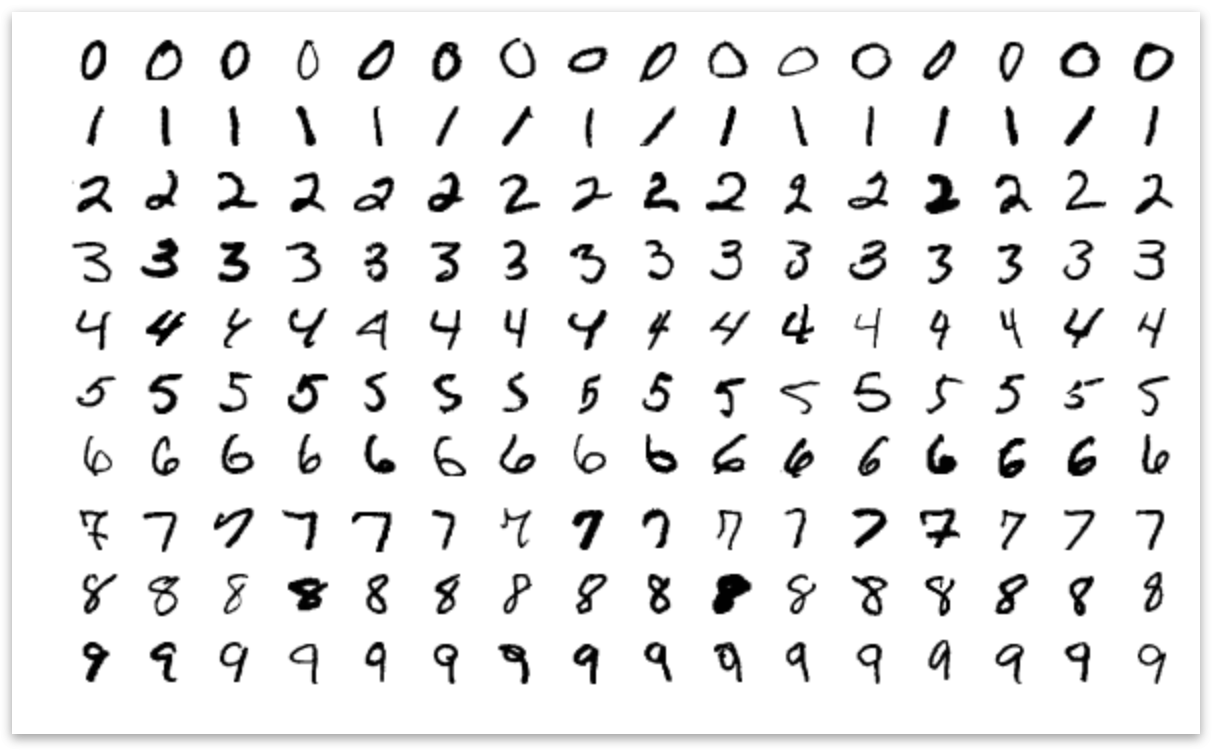
\includegraphics[width=0.5\textwidth]{Figures/Results/mnist.png}
  \caption[]{MNIST dataset example of handwritten digits.}
  \label{fig:mnist}
\end{figure}

The CNN was trained using the Radeon Vega Frontier Edition GPU, a top of the line graphics processor accelerator from AMD. This graphics card presents 8 levels of pairs of GPU Core frequency and voltage, Table \ref{tab:gpulevels}, that the GPU chooses in runtime accordingly to the temperature and power required, trying to maximize the performance. The GPU allows for the user definition of the frequency and voltage throw the ROCm System Management Interface - \textit{rocm-smi}. With it, a script was developed that performs undervoltage in steps of 10 mV on each of the 8 default voltage and frequency pairs. If the undervoltage is accepted by the software, the MNIST model is trained and after each run, the achieved accuracy is stored alongside the maximum power and average consumption, total energy consumed and the time that it took to execute the train.







\begin{figure}[!htb]
  \centering
  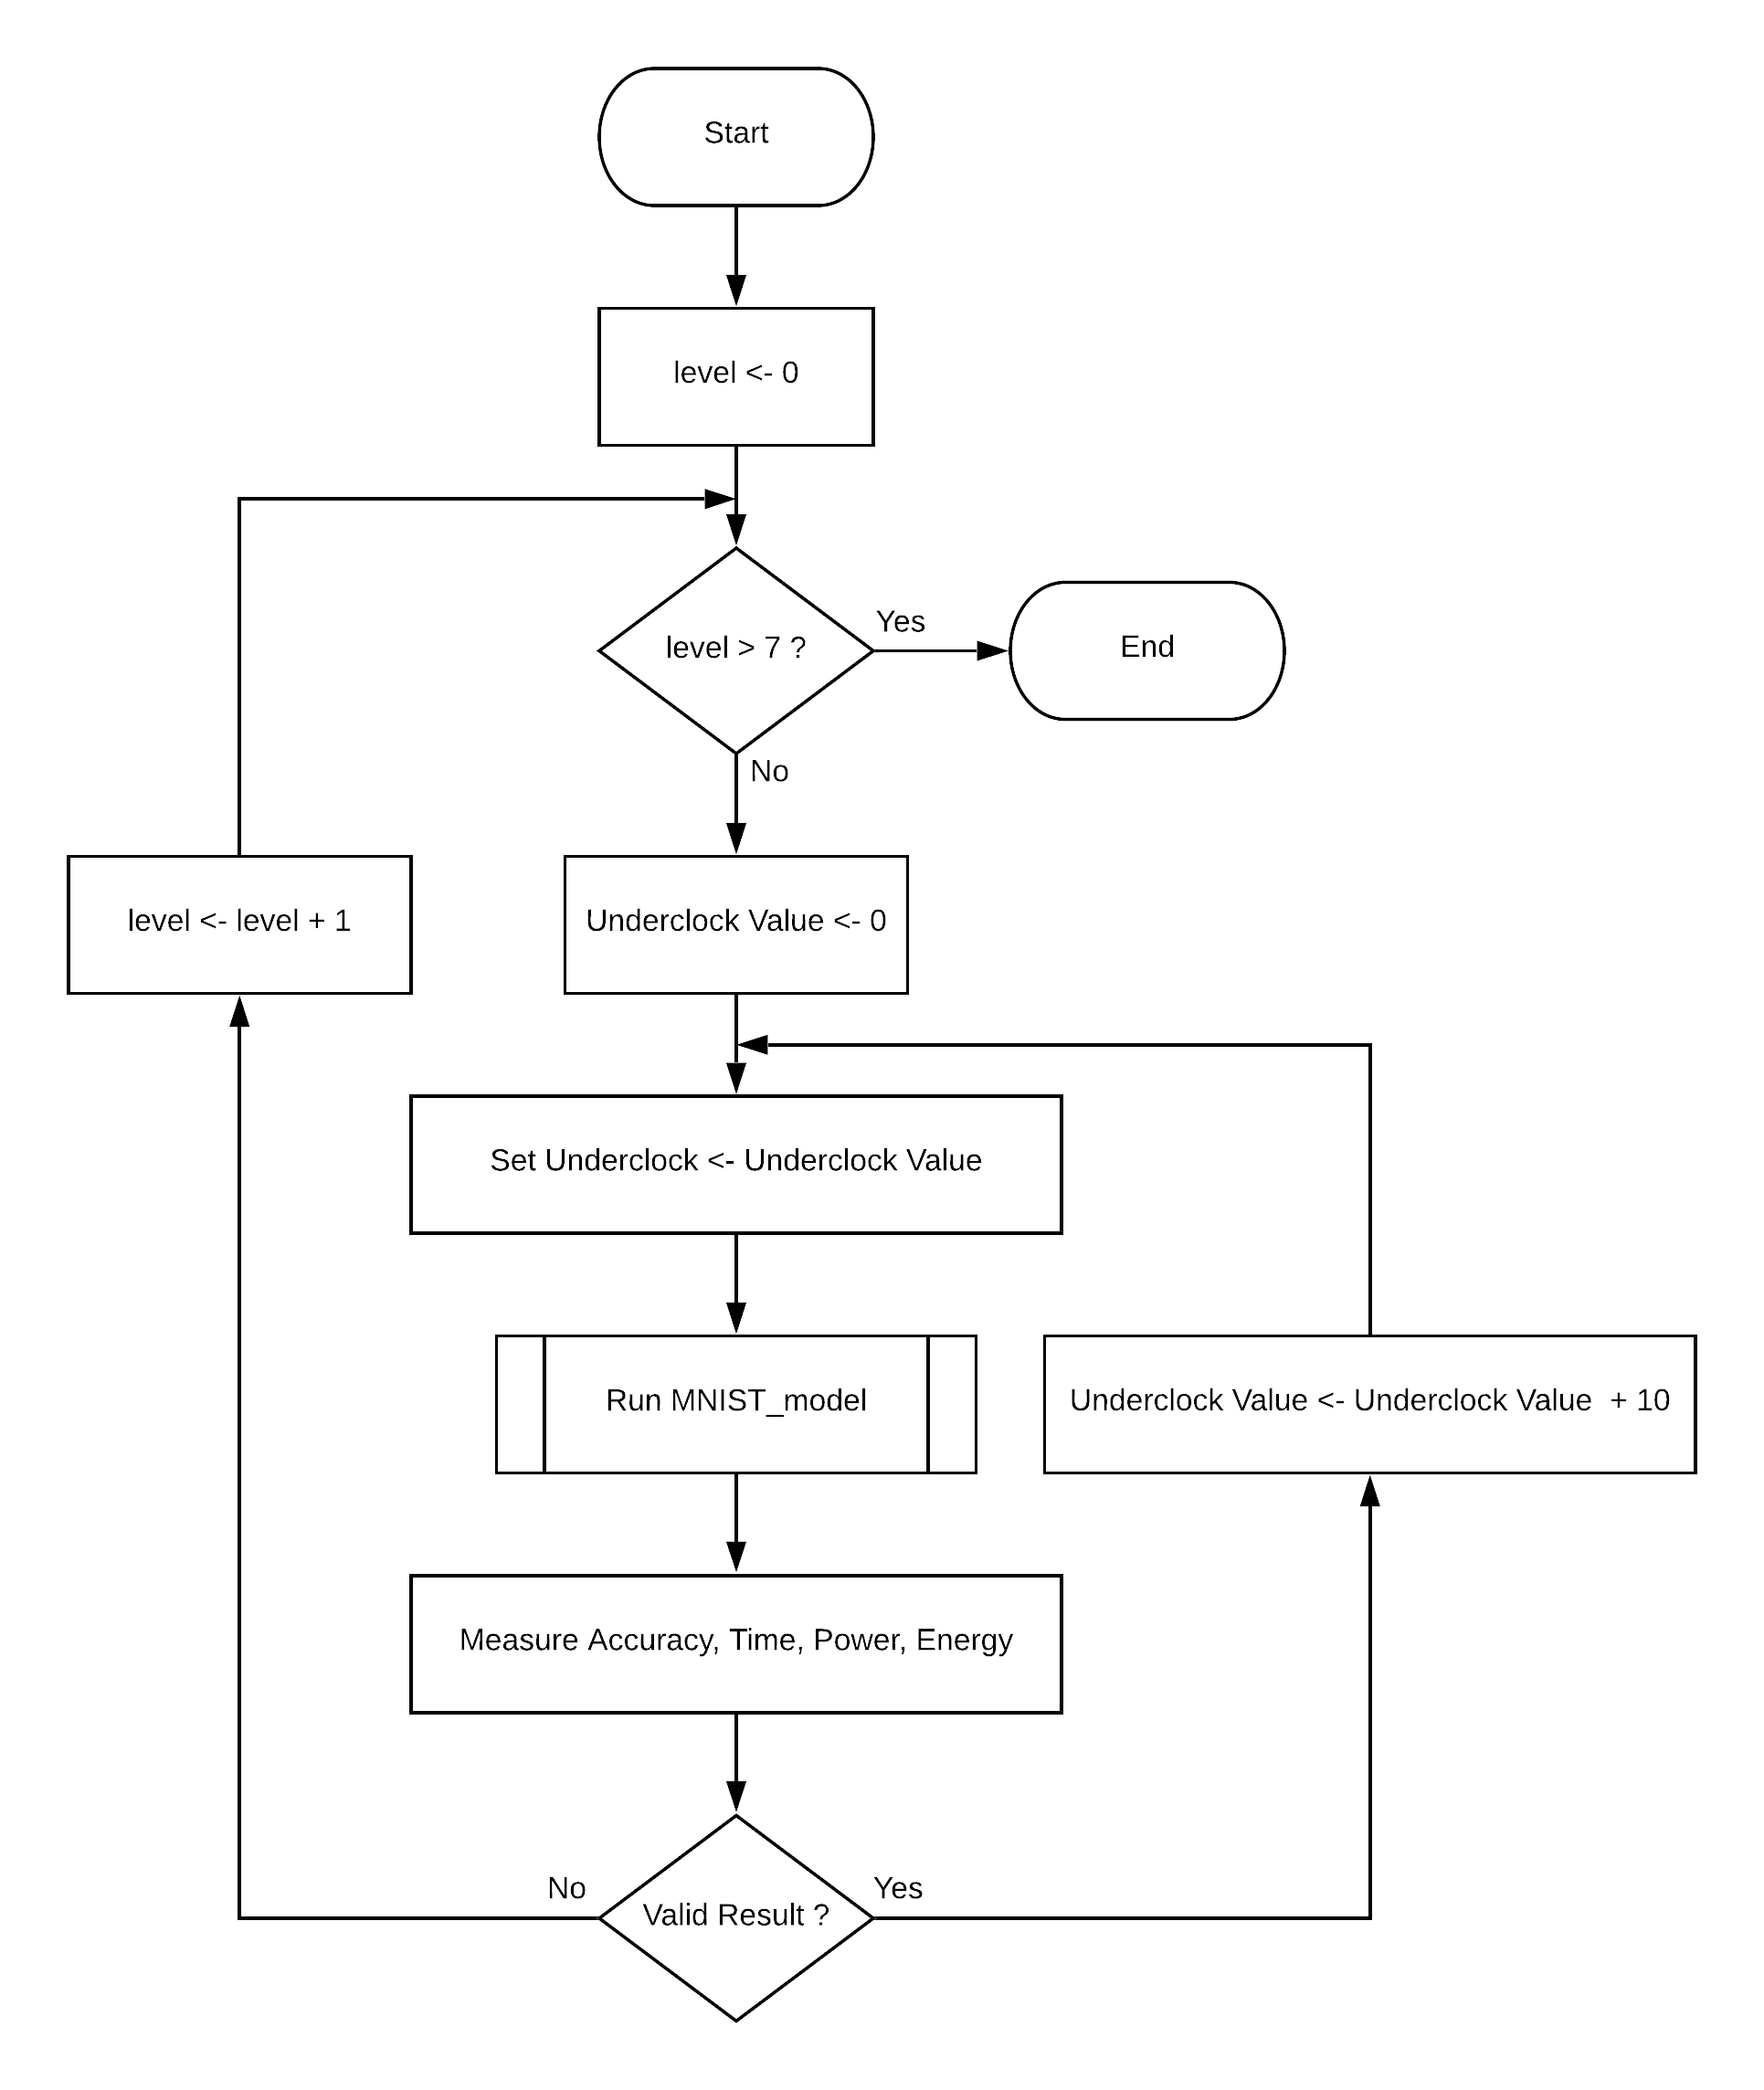
\includegraphics[width=0.75\textwidth]{Figures/Results/Underclock_Program.png}
  \caption[]{Flowchart of Automation Undervoltage Script.}
  \label{fig:undervoltage_program}
\end{figure}





\subsection{Preleminary Results}
\label{section:dvfseffects}

%%%%%%%%%%%%%%%%%%%%%%%%%%%%%%%%%%%%%%%%%%%%%%%%%%%%%%%%%%%%%%%%%%%%%%%%
\subsubsection{OverClock}
\label{section:underclock}

\subsubsection{UnderVoltage}




